\documentclass[preprint,12pt]{elsarticle}


%% The `ecrc' package must be called to make the CRC functionality available
%\usepackage{ecrc}

%% set the volume if you know. Otherwise `00'
%\volume{00}

%% set the starting page if not 1
%\firstpage{1}

%% Give the name of the journal
%\journalname{Expert Systems With Applications}

%% Give the author list to appear in the running head
%% Example \runauth{C.V. Radhakrishnan et al.}
%\runauth{}

%% The choice of journal logo is determined by the \jid and \jnltitlelogo commands.
%% A user-supplied logo with the name <\jid>logo.pdf will be inserted if present.
%% e.g. if \jid{yspmi} the system will look for a file yspmilogo.pdf
%% Otherwise the content of \jnltitlelogo will be set between horizontal lines as a default logo

%% Give the abbreviation of the Journal.  Contact the journal editorial office if in any doubt
%\jid{eswa}

%% Give a short journal name for the dummy logo (if needed)
%\jnltitlelogo{ESWA Logo}

%% Provide the copyright line to appear in the abstract
%% Usage:
%   \CopyrightLine[<text-before-year>]{<year>}{<restt-of-the-copyright-text>}
%   \CopyrightLine[Crown copyright]{2011}{Published by Elsevier Ltd.}
%   \CopyrightLine{2011}{Elsevier Ltd. All rights reserved}
%\CopyrightLine{2013}{Published by Elsevier Ltd.}



%\usepackage{llncsdoc}
\usepackage[figuresright]{rotating}
%\usepackage{makeidx}  % allows for indexgeneration
\usepackage{graphicx}
\usepackage[T1]{fontenc}
\usepackage[english]{babel}
\usepackage[utf8]{inputenc}
% \usepackage{multirow}

\usepackage{url}
\usepackage{rotating}

%%%Math
\usepackage{latexsym}
 \usepackage{amsmath}
% \usepackage{amssymb}
% \usepackage{amsthm}
%\usepackage{eurosans}

\usepackage{eurosym}

\usepackage{longtable}

\usepackage{listings}

\usepackage{color}
\usepackage{textcomp}


\definecolor{gray}{gray}{0.5}
\definecolor{green}{rgb}{0,0.5,0}
% 
% \usepackage{inconsolata}



\begin{document}


\begin{frontmatter}

%% Title, authors and addresses

%% use the tnoteref command within \title for footnotes;
%% use the tnotetext command for the associated footnote;
%% use the fnref command within \author or \address for footnotes;
%% use the fntext command for the associated footnote;
%% use the corref command within \author for corresponding author footnotes;
%% use the cortext command for the associated footnote;
%% use the ead command for the email address,
%% and the form \ead[url] for the home page:
%%
%% \title{Title\tnoteref{label1}}
%% \tnotetext[label1]{}
%% \author{Name\corref{cor1}\fnref{label2}}
%% \ead{email address}
%% \ead[url]{home page}
%% \fntext[label2]{}
%% \cortext[cor1]{}
%% \address{Address\fnref{label3}}
%% \fntext[label3]{}

%\dochead{}
%% Use \dochead if there is an article header, e.g. \dochead{Short communication}
%% \dochead can also be used to include a conference title, if directed by the editors
%% e.g. \dochead{17th International Conference on Dynamical Processes in Excited States of Solids}


\title{Semantic-based QoS management in Cloud Systems: Current Status and Future Challenges}


%% use optional labels to link authors explicitly to addresses:
% \author[label1]{Jose María Alvarez-Rodríguez\corref{cor1}}
% \address[label1]{The South East European Research Center, Thessaloniki, Greece.}
% \ead{jmalvarez@seerc.org}
% \ead[url]{http://www.seerc.org}
% 
% \author[label2]{José Emilio Labra-Gayo}
% \address[label2]{WESO Research Group, Department of Computer Science, University of Oviedo, 33007, Oviedo, Spain.}
% \ead{labra@uniovi.es}
% 
% \author[label3]{Alejandro Rodríguez-González}
% \address[label3]{Bioinformatics at Centre for Plant Biotechnology and Genomics UPM-INIA, Polytechnic University of Madrid, Madrid, Spain.}
% \ead{alejandro.rodriguezg@upm.es}
% 
% \author[label4]{Patricia Ordoñez De Pablos}
% \address[label4]{WESO Research Group, Department of Business Administration, University of Oviedo, 33007, Oviedo, Spain.}
% \ead{patriop@uniovi.es}





\author{}

\address{}

\begin{abstract}
The concept of Cloud Computing and Service Oriented Architectures have seen a 
dramatic increase of the amount of applications, services, management platforms, 
data, etc. gaining momentum in Information and Communication Technology and more 
specifically in the deployment of the Future Internet. However this explosion 
implies the necessity of new complex methods and techniques to deal with the 
vast heterogeneity of data sources, services or platforms. In this sense Quality 
of Service (QoS) seeks for providing an intelligent environment of 
self-management components based on domain knowledge in which both functional 
and nonfunctional properties of cloud components can be optimized in terms of 
cost, efficiency or reliability easing the transition to an advanced resource 
provisioning process. On the other hand, semantics and ontologies have emerged 
as part of the Artificial Intelligence to afford a common and standard data 
model that ease the interoperability, integration and monitorization of 
knowledge-based systems. Furthermore the Linked Data initiative as practical 
view of the Semantic Web has posed the baseline technology to easily integrate, 
enrich and consume data in a distributed system. Taking into account the 
necessity of an intelligent system to manage QoS in Cloud Systems and the 
emerging application of semantics, ontologies and Linked Data in different 
domains, this paper reviews the main approaches for semantic-based QoS 
management as well as the principal methods, techniques and standards for 
processing and exploiting diverse data providing advanced real-time monitoring 
services for QoS. A discussion of existing efforts and challenges are also 
provided to suggest future directions.
\end{abstract}

\begin{keyword}
%% keywords here, in the form: keyword \sep keyword
cloud systems \sep quality of service \sep  service oriented architectures \sep  semantics \sep  ontologies \sep  linked data \sep  sensor data \sep  big data 
%% PACS codes here, in the form: \PACS code \sep code

%% MSC codes here, in the form: \MSC code \sep code
%% or \MSC[2008] code \sep code (2000 is the default)

\end{keyword}


\end{frontmatter}

\section{Introduction}
Cloud Computing~\cite{mell2011nist} systems and Service Oriented Architectures (SOA) have 
reached a level of complexity~\cite{Huebscher:2008:SAC:1380584.1380585,Conejero:2012:MSQ:2357487.2357591} that implies the necessity of new methods 
and algorithms to automatically deal with the vast amount of data, variables, 
parameters, etc. that appear in this new realm for the advanced management of 
applications, services or resources. 

In this new environment QoS is playing a relatively minor role but its 
importance, in a wide range of applications scenarios, is likely become more 
crucial than ever before. In recent years and due to the deployment of web 
services a considerable research effort in QoS has been made. However existing 
QoS mechanisms are actually available in a few large scale commercial 
environments and with a limited extent. The main problem lies in the complexity 
of designing QoS models that enables an adequate management of a distributed 
architecture making decisions about resource provisioning, getting feedback for 
the final users, etc. with the objective of avoiding existing ``brute-force''
solutions and overprovisioning. 

Although QoS management has been also widely investigated~\cite{Conejero:2012:MSQ:2357487.2357591} 
in the well-known grid-computing area the emergence of the Cloud Computing paradigm 
brings a new set of open issues: accomplish the  Service Level Agreements (SLAs), predict 
future workload, process large and diverse data streams/logs, make real-time 
decisions, reasoning and inference, dynamic adaptation and provision of 
resources, etc. In the widely-accepted definition~\cite{mell2011nist} of 
he National Institute of Standards and Technology (NIST) QoS 
would be aligned to the concept of ``Measured Service'', see Figure~\ref{fig:qos-intro}, and 
more specifically to define both characteristics applicable to a service and operations 
to deliver some kind of alert or predictive analytics service. 
The aforementioned points are very challenging and should be 
addressed in order to ease an intelligent, flexible and self-managing system of 
cloud-based applications and platforms.


 \begin{figure}[!ht]
\centering
	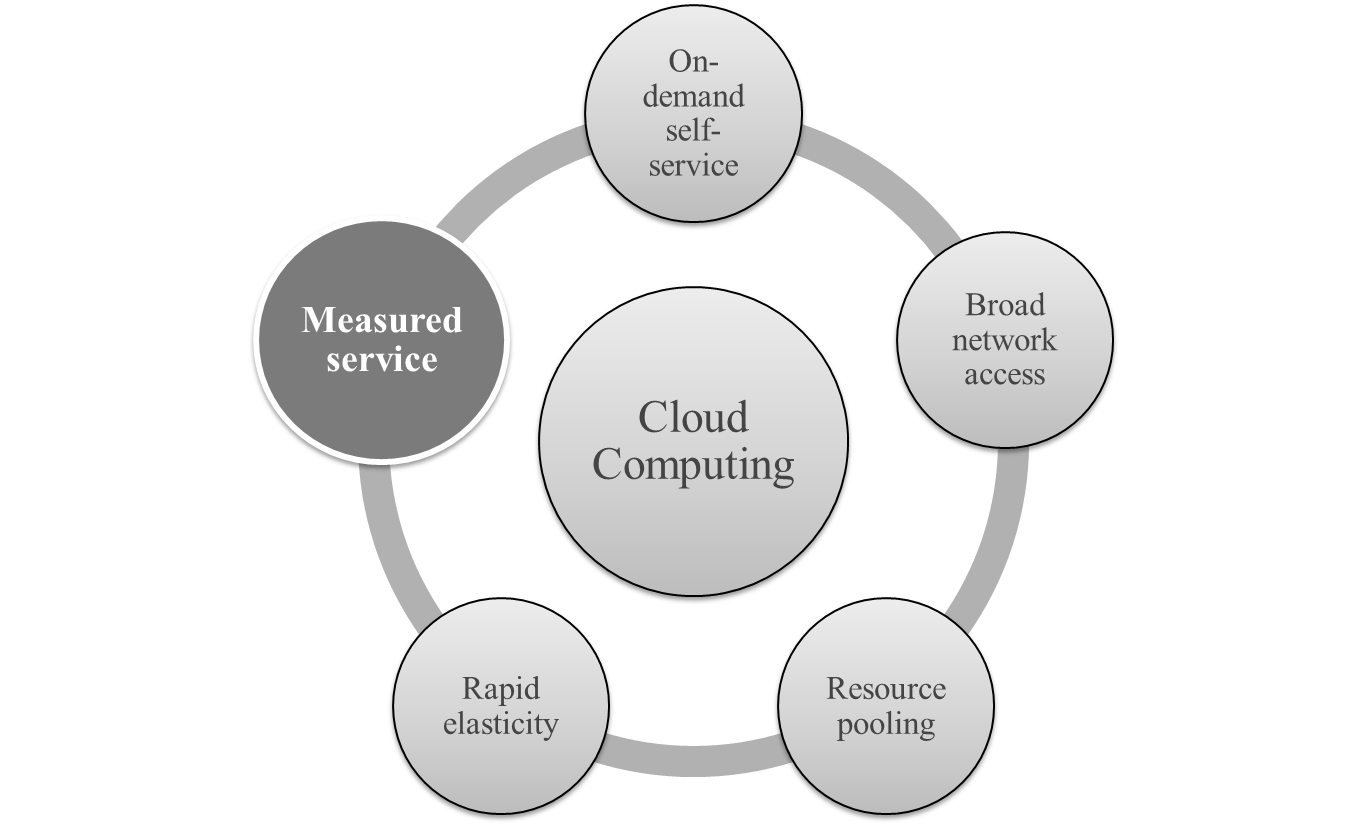
\includegraphics[width=12cm]{./imgs/qos-intro}
 \caption{Quality of Service in the NIST definition~\cite{mell2011nist}.}
 \label{fig:qos-intro}
\end{figure}

Furthermore a proper management of a cloud system taking into account QoS 
features can save costs, keep high-performance, reserve resources on-demand and 
offer a user-friendly experience to both IT managers and final users. 
Traditionally, QoS has been handled using a combination of network resource 
provisioning with techniques such as admission control or active queue 
management. Nowadays these old-fashioned techniques can be applied to a static 
environment but in the future, the challenge of providing higher elasticity and 
dynamic adaptation cannot be accomplished with these methods. In this sense it 
is clear that QoS will remain a fundamental requirement in the next wave of 
applications and services on the Web and there is no doubt that QoS should 
address the new challenges applying emerging and trending technology and 
approaches to overcome existing restrictions in QoS models.

The features and requirements of these new cloud systems with regards 
to QoS~\cite{Pedersen:2011:AMQ:2114495.2115542} match the advantages of software component and 
knowledge-based architectures. In fact, Autonomic Computing support for the next generation of cloud systems 
needs to be~\cite{Conejero:2012:MSQ:2357487.2357591,Pedersen:2011:AMQ:2114495.2115542}: 
1) Self-x management, 2) agile, flexible and reliable, 4) deployable over a multiple cloud platforms, 5) handle complexity, 6) enable 
collaboration and coordination and 7) cost-effective and greener 
(energy-efficient). Under this context, semantic technologies have emerged as an 
option to design and develop intelligent software components and agents to 
perform certain tasks on the Web and fulfill user's requirements (in this case 
applications). Therefore, Semantics enables machines to automatically process 
and enrich data from different sources and has the potential to deeply influence 
the further development of the Internet Economy as cloud systems also does.

In the Semantic Web area, there is a growing commitment to process large data streams applying 
new stream reasoning~\cite{Bolles:2008:SSE:1789394.1789438,Barbieri:2010:EEC:1739041.1739095} 
or complex event processing (CEP) techniques~\cite{Anicic:2011:EUL:1963405.1963495}. Furthermore there are research works offering cloud-based 
solutions to deal with Big Data~\cite{Fan:2013:MBD:2481244.2481246} (e.g. analysis of social media), modeling SLAs and ECA rules with ontologies, 
monitoring real-time systems (e.g. traffic), sensor networks, or making decisions in a collaborative fashion~\cite{RodriGuez-GonzaLez:2012:UAP:2350799.2350907} (e.g. clinical reasoning). 
The main advantage of applying semantic technologies to a specific domain lies in the standard representation of knowledge and data through a common-shared data model (RDF) and the 
capacity of reusing existing knowledge through ontologies (OWL). Thus, data coming from cloud systems can be automatically processed, checked for inconsistencies and 
used in expert systems to support self-x management activities.

This review is intended to provide researchers, developers and practitioners a summary of the current status of QoS management in Cloud Computing and SOA applying semantics. To do so, the paper 
is structured as follows. Next section reviews the background concepts required to a better understanding of the paper. Section~\ref{qos-semantics} 
presents the existing works to perform QoS management using semantics; more specifically most of the ontology-based frameworks for 
QoS management are reviewed. Afterwards, a review of existing techniques for processing large data streams is also provided in Section~\ref{data-stream}. 
Section~\ref{framework} outlines a framework to meet QoS requirements applying semantics and data strea processing techniques in real-time. 
Finally, the paper ends with an evaluation, discussion of existing approaches for semantic-based QoS management, 
limitations, future challenges and concluding remarks. 


\section{Background}
This section presents a brief summary of the background concepts reviewed in this paper: 
1) Cloud Computing and QoS; 2) Semantic Technologies and 3) Big Data, with the 
aim of building a common understanding of the requirements of QoS in Cloud Computing.


\subsection{Quality of Service in Cloud Systems}\label{qos-cloud-index}
Cloud Computing represents the next natural step in the evolution of on-demand services and applications. 
Several definitions have been made but the description~\cite{mell2011nist} provided by the NIST institute has reached a major consensus:  
``A large-scale distributed computing paradigm that is driven by economies of scale, in which a pool of 
abstracted, virtualized, dynamically-scalable, managed computing power, storage, platforms, and services are delivered on demand to external customers over the Internet''. 
The NIST institute has also defined~\cite{mell2011nist,Garcia-Sanchez:2010:ASS:1852403.1852409}: 
\begin{enumerate}
 \item Five key characteristics: on-demand self-service, ubiquitous network access, location independent resource pooling, rapid elasticity and pay per use.
 \item Three service models: Software-as-a-Service (SaaS), Platform-as-a-Service (PaaS) and Infrastructure-as-a-Service (IaaS).
 \item Four development models: private, community, public and hybrid clouds. 
\end{enumerate}

These basic concepts~\cite{mell2011nist} and usages~\cite{cloud-usage} in a cloud environment lead us to consider that QoS is a key-enabler of the five essential characteristics identified by 
the NIST institute and it is closely related to the concepts of Autonomic and Utility Computing~\cite{Huebscher:2008:SAC:1380584.1380585}. 
As a consequence the QoS management is clearly a key-enabler of cloud environments and it must play a major role in the Future Internet to 
afford, from a quality point of view, the implementation of the ``Measured Service'' concept, see Figure~\ref{fig:qos-intro}.

On the other hand, the ITUT-T Recommendation E.800 defines QoS as ``collective effect of service performance that determines the degree of 
satisfaction by a user of the service''. Thus QoS data is a key-enabler to design, identify and put in action SLAs. It should also influence 
software components and applications to ensure a reliable environment for executing services. Some open issues in 
QoS management emerge to extend this definition including reputation-based mechanisms for service selection or 
dynamic adaptation of resource provisioning. The application of QoS has been widely studied and 
applied~\cite{Conejero:2012:MSQ:2357487.2357591,Pedersen:2011:AMQ:2114495.2115542} to web services and grid computing areas and it is now 
gaining momentum in the new Cloud Computing paradigm. 

In order to facilitate the QoS management in the cloud-environment some tools, called Cloud Management Platforms (CMPs) can be found 
to manage the different layers of cloud-based applications but the majority of them are now focused on the IaaS layer. 
The use of these platforms can help to manage the growing of cloud applications and ease the deployment and monitoring of services across 
public and private clouds. The six key capabilities~\cite{Kephart2012} that we should look for in a CMP are: simplify complexity, 
manage multiple clouds, build for the future, support the whole application lifecycle, self-management (set-it and forget-it) and manage/control costs. 
In this sense OASIS just launched a CAMP TC~\cite{OASISCamp} to create and inter-operable protocol that cloud 
implementers can use to package and deploy their applications. The idea is to provide a set of REST services, at the PaaS layer, to foster an ecosystem of 
common tools, plug-ins, libraries and frameworks, which will allow vendors to offer greater value-add. In the particular case of QoS, the use of standards to gather data 
from applications can improve the process of making decisions about resource provisioning or help in saving costs among others. Nevertheless 
this specification is still in an early stage and its objectives are more focused on the management of cross-cloud applications than a 
real management from QoS point of view. Following main characteristics of the CAMP specification are presented:
\begin{itemize}
 \item It is a language, framework and platform neutral to manage in the same way Java, Ruby on Rails or Node.js applications.
 \item It only covers interactions between a cloud consumer and a provider~\cite{mell2011nist}.
 \item It supports the management of the entire lifecycle of the application not just the deployment of isolated components.
 \item A major objective of the specification is to provide an inter-operable environment. They are trying to keep simple as 
 possible but with the possibility of being extended by third-parties.
\end{itemize}

Although there is no a clear objective to support quality indicators it can be considered as a major effort to unify information exposed by providers and 
improve the creation of an integrated and inter-operable ecosystem in which existing cloud management application platforms such 
as RightScale, Enstratus, ScaleUp, Cloudability, Cloudyn, CloudExpress or MyGravitant can take advantage of implemented 
added-value services on the top of a common API. Although these commercial products offer a very good option 
to manage cloud-based applications there is a lack of standardization and some QoS features cannot be managed.  
Nevertheless these existing cloud management platforms present some interesting features and services for 
multi-cloud management that must be taken into account in the design of a dedicated cloud quality management platform such as:
\begin{itemize}
 \item Integrated management of cloud resources: compute, networking and storage.
 \item Organization: tagging capabilities or creation of profiles and views to group cloud resources.
 \item Accessibility and usability: monitoring (tracking and graphing custom metrics), dashboard or import capabilities.
 \item Custom services: creation of alerts using a particular set of indicators, cost forecasting or reporting.
\end{itemize}

%Policy making
On the other hand there is an interesting approach to manage cloud quality indicators using a policy-making 
perspective. In this sense public and private bodies are continuously seeking for new analytical tools and methods to 
assess, rank and compare their performance based on distinct indicators and dimensions with the objective of making 
some decision or developing a new policy. In this context the creation and use of quantitative indexes is 
a widely accepted practice that has been applied to various domains such as Bibliometrics and academic performance and 
quality (the Impact Factor by Thomson-Reuters, the H-index or the Shanghai and Webometrics rankings) the Web impact (the Webindex~\cite{webindexlod} 
by the Webfoundation) or Smart Cities (The European Smart Cities ranking) to name a few. Therefore policymakers as well as individuals are 
continuously evaluating quantitative measures to tackle or improve existing problems in different areas and 
support their decisions. Nevertheless the sheer mass of data now available is raising a new dynamic and challenging environment 
in which traditional tools are facing major problems to deal with data-sources diversity, structural issues or complex processes of estimation. 
According to some efforts such as the ``Policy-making $2.0$'' within the Cross-Over project~\footnote{\url{http://www.crossover-project.eu/}} 
that \textit{refers to a blend of emerging and fast developing technologies that enable better, more timely and more participated decision-making}, 
new paradigms and tools are required to take advantage of the existing environment (open data and big data) to design and estimate 
actions in this dynamic context according to requirements of transparency, standardization, adaptability and extensibility among 
others with the aim of providing new context-aware and added-value services such as visualization that 
can help a deepen and broaden understanding of the impact of a policy in a more fast and efficient way. 
As a consequence common features and requirements can be extracted from the existing situation out:
\begin{itemize}
 \item Data sources. Data and information is continuously being generated as observations from social networks, public and private institutions, NGOs, services and applications, etc. 
 creating a tangled environment of sources, formats and access protocols with a huge but restricted potential for exploitation. Nevertheless data processing, knowledge inferring, etc. are not mere processes 
 of gathering and analyzing, it is necessary to deal with semantic and syntactic issues, e.g. particular measurements and dimensions or name mismatches, 
 in order to enable a proper data/information re-use and knowledge generation.
 
 \item Structure. Quantitative indexes are usually defined (a mathematical model) by experts to aggregate several indicators (in a hierarchy structure) 
 in just one value to provide a measure of the impact or performance of some policy in a certain context. The structure of these indexes are 
 obviously subjected to change over time  to collect more information or adjust their composition and relationships (narrower/broader). 
 That is why technology should be able to afford adequate techniques to automatically populate new changes in an efficient way.
 
  \item Computation process. This feature refers to the calculation of the index. Observations are gathered from diverse data sources and aligned 
  to the index structure, commonly indicators, that are processed through various mathematical operators to generate a final index value. 
  Nevertheless the computation process is not always described neither open (any minor change can imply a long time for validation) implying that 
  cannot be easily replied for third-parties with other purposes, for instance research, preventing one 
  of the most wanted characteristics such as transparency. Furthermore it is necessary to ensure that the computation process 
  is sound and correct.

  \item Documentation. As the European project Cross-over has stated, new policy-making strategies go ahead of a simple and closed value and it is necessary to bring 
  new ways of exploiting data and information. Moreover the use of the Web as a dissemination channel represents a powerful environment in which 
  information should be available taking into account the multilingual and multicultural character of information. In this context documentation mechanisms 
  must necessarily cover all the aforementioned features to afford a detailed explanation of a quantitative index-based policy to both policymakers 
  and final users. However existing initiatives usually generates some kind of hand-made report which is not easy to keep up-to-date and deliver 
  to the long-tail of interested third-parties.
\end{itemize}

Following this perspective of creating a quantitative index the Cloud Computing community~\cite{Maiya:2012:QMC:2353730.2353862,DBLP:conf/quatic/KlemsBW12} 
and some of the big players have launched some relevant indexes such as:

\begin{itemize}
 \item The Service Measurement Index~\cite{smi} by the Cloud Services Measurement Initiative Consortium (CSMIC) consortium. It is 
 based on a framework of critical key performance indicators (both business and technical) \textit{associated attributes, and measures 
 that provide a standardized method for measuring and comparing a business service regardless of whether that service is internally provided or sourced from an outside company for any cloud service (IaaS, PaaS, SaaS, etc.). It is designed to become a 
 standard method to help organizations measure cloud-based services based on their specific business and technology requirements.} As 
 an implementation of the SMI Index the ``Ranking Clouds''~\cite{DBLP:journals/fgcs/GargVB13} presents a framework to manage this index 
 and makes a ranking of different PaaS providers using the AHP method to weight some key performance indicators.
 
 \item The Cisco Global Cloud Index (GCI) by Cisco~\cite{cisco}. \textit{It is an ongoing effort to forecast the growth of global data 
 center and cloud-based IP traffic. The forecast includes trends associated with data center virtualization and cloud computing. }
 It also provides a visual representation of countries ranging  from ``Cloud Prepared'' to ``Cloud Emerging''.

 \item The CSC Cloud Usage index~\cite{csc}. It is an index created through a survey of more than ·$3500$ cloud computing users 
 in eight countries around the world. The survey is focused on capturing user information about outcomes and 
 experiences rather than predictions and intentions.

 \item The VMWare Cloud index~\cite{vmware}. It is an study conducted by Forrester Consulting and ITR in Japan. \textit{The 2012 study surveyed 
 approximately $6500$ senior IT practitioners across the APJ region in eleven countries / regions with the aim of establishing 
 top cloud drivers and concerns in the community.}

\end{itemize}

FIXME: some concluding remarks?

% 
% 
% \begin{sidewaystable}[!ht]
% \renewcommand{\arraystretch}{1.3}
% \tiny
% \begin{center}
% \begin{tabular}[c]{|p{2.5cm}|p{9cm}|p{1.5cm}|p{1.5cm}|p{1.5cm}|} 
% \hline
%   \textbf{KPI} &  \textbf{Definition}  &  \textbf{Broader} & \textbf{Defined by} & \textbf{Scope} \\\hline
%   Accountability&This component is used to measure the properties related to the service provider
% organization. These properties may be independent of the service being provided.&&CSMIC&$\ast$ \\ \hline
%   Agility&Indicates the impact of a service upon a client's ability to change direction, strategy, or tactics quickly and with minimal disruption.&&CSMIC&$\ast$ \\ \hline
%   Assurance&This category includes key attributes that indicate how likely it is that the service will be available as specified.&&CSMIC&$\ast$ \\ \hline 
%   Financial&The amount of money spent on the service by the client.&&CSMIC&$\ast$ \\ \hline 
%   Performance&This category covers the features and functions of the provided services.&&CSMIC&$\ast$ \\ \hline 
%   Security and Privacy&This category includes attributes that indicate the effectiveness of a service provider's controls on access to services, service data, and the physical facilities from which services are provided.&&CSMIC&$\ast$ \\ \hline 
%   Usability&The ease with which a service can be used.&&CSMIC&$\ast$ \\ \hline 
%   Auditability&The ability of a client to verify that the service provider is adhering to the standards, processes, and policies that they follow.&Accountability&CSMIC&$\ast$ \\ \hline 
%   Compliance&Standards, processes, and policies committed to by the service provider are followed.&Accountability&CSMIC&$\ast$ \\ \hline 
%   Contracting Experience&Indicators of client effort and satisfaction with the process of entering into the agreements required to use a service.&Accountability&CSMIC&$\ast$ \\ \hline 
%   Data Ownership&The Level of rights a client has over client data associated with a service.&Accountability&CSMIC&$\ast$ \\ \hline 
%   Ease of Doing Business&Client satisfaction with the ability to do business with a service provider.&Accountability&CSMIC&$\ast$ \\ \hline 
%   Ease of Doing Business&The processes used by the service provider to manage client expectations, issues and service performance.&Accountability&CSMIC&$\ast$ \\ \hline 
%   Ownership&The level of rights a client has over software licenses, intellectual property and data associated with a service.&Accountability&CSMIC&$\ast$ \\ \hline 
%   Provider business stability&The likelihood that the service provider will continue to exist throughout the contracted term.&Accountability&CSMIC&$\ast$ \\ \hline 
%   Provider Certifications&The service provider maintains current certifications for standards relevant to their clients' requirements.&Accountability&CSMIC&$\ast$ \\ \hline 
%   Provider Contract/SLA Verification&The service provider makes available to clients SLAs adequate to manage the service and mitigate risks of service failure.&Accountability&CSMIC&$\ast$ \\ \hline 
%   Provider Ethicality&Ethicality refers to the manner in which the service provider conducts business; it includes business practices and ethics outside the scope of regulatory compliance. Ethicality includes fair practices with suppliers, customers, and employees.&Accountability&CSMIC&$\ast$ \\ \hline 
%   Provider Personnel Requirements&The extent to which service provider personnel have the skills, experience, education, and certifications required to effectively deliver a service.&Accountability&CSMIC&$\ast$ \\ \hline 
%   Provider Supply Chain&The service provider ensures that any SLAs that must be supported by its suppliers are supported.&Accountability&CSMIC&$\ast$ \\ \hline 
%   Security Capabilities&The capabilities of service providers to ensure application, data, and infrastructure securiy based on the security requirements of the client.&Accountability&CSMIC&$\ast$ \\ \hline 
%   Sustainability&The impact on the economy, society and the environment of the service provider.&Accountability&SMIC&$\ast$ \\ \hline 
%   Adaptability&The ability of the service provider to adjust to changes in client requirements.&Agility&CSMIC&$\ast$ \\ \hline 
%   Capacity&The maximum amount of a service that a service provider can deliver while meeting agreed SLAs.&Agility&CSMIC&$\ast$ \\ \hline 
%   Elasticity&The ability of a service to adjust its resource consumption to meet demand.&Agility&CSMIC&$\ast$ \\ \hline 
%   Extensibility&The ability to add new features or services to existing services.&Agility&CSMIC&$\ast$ \\ \hline 
%   Flexibility&The ability to add or remove predefined features from a service.&Agility&CSMIC&$\ast$ \\ \hline 
%   Portability&The ability of a client to easily move a service from one service provider to another with minimal disruption.&Agility&CSMIC&$\ast$ \\ \hline 
%   Scalability&The ability of a service provider to increase or decrease the amount of service available to meet client requirements.&Agility&CSMIC&$\ast$ \\ \hline 
% \hline
% \end{tabular}
% \caption{Key Performance Indicators I.}\label{table:kpi-1}
%   \end{center}
% \end{sidewaystable} 
% 
% \begin{sidewaystable}[!ht]
% \renewcommand{\arraystretch}{1.3}
% \tiny
% \begin{center}
% \begin{tabular}[c]{|p{2.5cm}|p{9cm}|p{1.5cm}|p{1.5cm}|p{1.5cm}|} 
% \hline
%   \textbf{KPI} &  \textbf{Definition}  &  \textbf{Broader} & \textbf{Defined by} & \textbf{Scope} \\\hline
%  Availability&The amount of time that a client can make use of a service.&Assurance&CSMIC&$\ast$ \\ \hline 
%  Maintainability&Maintainability refers to the ability for the service provider to make modifications to the service to keep the service in a condition of good repair.&Assurance&CSMIC&$\ast$ \\ \hline 
%  Recoverability&Recoverability is the degree to which a service is able to quickly resume a normal state of operation after an unplanned disruption.&Assurance&CSMIC&$\ast$ \\ \hline 
%  Reliability&Reliability reflects measures of how a service operates without failure under given conditions during a given time period.&Assurance&CSMIC&$\ast$ \\ \hline 
%  Resiliency&The ability of a service to continue to operate properly in the event of a failure in one or more of its components.&Assurance&CSMIC&$\ast$ \\ \hline 
%  Stability&The degree to which the service is resistant to change, deterioration, or displacement.&Assurance&CSMIC&$\ast$ \\ \hline 
%  Serviceability&The ease and efficiency of performing maintenance and correcting problems with the service.&Assurance&CSMIC&$\ast$ \\ \hline 
%  Acquisition&Any client costs to acquire the rights and ability to use a service and to move from an existing service to the new one.&Financial&CSMIC&$\ast$ \\ \hline 
%  On-going Cost&The client cost to operate a service. This includes both recurring flat costs (e.g. monthly access fees) and usage-based costs.&Financial&CSMIC&$\ast$ \\ \hline 
%  Profit&Arrangement between client and provider(s) under which costs or profits of a service are shared by the involved parties, according to an agreed upon formula.&Financial&CSMIC&$\ast$ \\ \hline 
%  Accuracy&The extent to which a service adheres to its requirements.&Performance&CSMIC&$\ast$ \\ \hline 
%  Functionality&The specific features provided by a service.&Performance&CSMIC&$\ast$ \\ \hline 
%  Suitability&How closely do the capabilities of the service match the needs of the client.&Performance&CSMIC&$\ast$ \\ \hline 
%  Suitability&How closely do the capabilities of the service match the needs of the client.&Usability&CSMIC&$\ast$ \\ \hline 
%  Suitability&The ability of a service to easily interact with other services (from the same service provider and from other service providers).&Performance&CSMIC&$\ast$ \\ \hline 
%  Service Response Time&An indicator of the time between when a service is requested and when the response is available.&Performance&CSMIC&$\ast$ \\ \hline 
%  Access Control&Policies and processes in use by the service provider to ensure that only the provider and client personnel with appropriate status/reasons to make use of or modify data/work products may do so.&Security and Privacy&CSMIC&$\ast$ \\ \hline 
%  Geographical Constraint&The client's constraints on service location based on geography.&Security and Privacy&CSMIC&$\ast$ \\ \hline 
%  Political Constraint&The client's constraints on service location based on politics.&Security and Privacy&CSMIC&$\ast$ \\ \hline 
%  Data Integrity&Keeping the data that is created, used, and stored in its correct form so that clients may be confident that it is accurate and valid.&Security and Privacy&CSMIC&$\ast$ \\ \hline 
%  Data Privacy&Client restrictions on access and use of client data are enforced by the service provider. Any failures of these protections are promptly detected and reported to the client.&Security and Privacy&CSMIC&$\ast$ \\ \hline 
%  Data Loss&Client restrictions on access and use of client data are enforced by the service provider. Any failures of these protections are promptly detected and reported to the client.&Security and Privacy&CSMIC&$\ast$ \\ \hline 
%  Physical \& Environmental Security&Policies and processes in use by the service provider to protect the provider facilities from unauthorized access, damage or interference.&Security and Privacy&CSMIC&$\ast$ \\ \hline 
%  Proactive Threat \&  Vulnerability Management&Mechanisms in place to ensure that the service is protected against know recurring threats as well as new evolving vulnerabilities.&Security and Privacy&CSMIC&$\ast$ \\ \hline 
%  Retention/Disposition&The service provider’s data retention and disposition processes meet the clients' requirements.&Security and Privacy&CSMIC&$\ast$ \\ \hline 
%  Accessibility&The degree to which a service is operable by users with disabilities.&Usability&CSMIC&$\ast$ \\ \hline 
%  Client Personnel Requirements&The minimum number of personnel satisfying roles, skills, experience, education, and certification required of the client to effectively utilize a service.&Usability&CSMIC&$\ast$ \\ \hline 
%  Client Personnel Requirements&Installability characterizes the time and effort required to get a service ready for delivery (where applicable).&Usability&CSMIC&$\ast$ \\ \hline 
%  Learnability&The effort required of users to learn to use the service.&Usability&CSMIC&$\ast$ \\ \hline 
%  Operability&The ability of a service to be easily operated by users.&Usability&CSMIC&$\ast$ \\ \hline 
%  Transparency&The extent to which users are able to determine when changes in a feature or component of the service occur and whether these changes impact usability.&Usability&CSMIC&$\ast$ \\ \hline 
%  Understandability&The ease with which users can understand the capabilities and operation of the service.&Usability&CSMIC&$\ast$ \\ \hline 
% 
% \hline
% \end{tabular}
% \caption{Key Performance Indicators II.}\label{table:kpi-2}
%   \end{center}
% \end{sidewaystable} 
% 

\subsection{Semantic Technologies}
The Semantic Web area, coined by Tim Berners-Lee in 2001, has experienced during last years a growing 
commitment from both academia and industrial areas  with the objective of elevating the meaning of web 
information resources through a common and shared data model (graphs) and an underlying semantics based 
on different logic formalisms (ontologies). The Resource Description Framework (RDF), based on a graph model, and the Web Ontology Language (OWL), 
designed to formalize and model domain knowledge, are the two main \textit{ingredients} to reuse information and data 
in a knowledge-based realm. Thus data, information and knowledge can be easily shared, exchanged and linked~\cite{Maali_Cyganiak_2011} 
to other knowledge-based systems and databases through the use URIs, more specifically HTTP-URIs. Therefore the broad objective of this effort can be summarized 
as a new environment of added-value information and services that can boost and improve B2B (Business to Business), B2C (Business to Client) or 
A2A (Administration to Administration) relationships. The implementation of new context-awareness expert systems to tackle existing 
cross-domain problems such as medical reasoning, analysis of social media, etc. in which data heterogeneities, 
lack of standard knowledge representation and interoperability problems are common factors that the use of semantics can improve. As a practical view of the Semantic Web, 
the Linked Data~\cite{Berners-Lee-2006,Heath_Bizer_2011} initiative emerges to create a large and distributed database on the Web. 
In order to reach this major objective the publication of information and data under a common data model (RDF) 
with a specific formal query language (SPARQL~\cite{Sparql11}) provides the required building blocks to turn the Web of documents 
into a real database or ``Web of Data''. Research works are focused in two main areas: 1) production/publishing~\cite{bizer07how} and 2) consumption of 
Linked Data. In the first case data quality~\cite{bizer2007,Bizer2009QA,lodq,link-qa}, conformance~\cite{DBLP:journals/ws/HoganUHCPD12}, 
provenance~\cite{w3c-prov,DBLP:conf/ipaw/HartigZ10}, trust~\cite{Carroll05namedgraphs}, description of 
datasets~\cite{void,Cyganiak08semanticsitemaps,ckanValidator} and entity reconciliation~\cite{Serimi,Maali_Cyganiak_2011} issues are 
becoming major objectives since a mass of amount data is already available through RDF repositories and SPARQL endpoints. 

On the other hand, consumption of Linked Data is being addressed to provide new ways of data 
visualization~\cite{DBLP:journals/semweb/DadzieR11,hoga-etal-2011-swse-JWS}, faceted browsing~\cite{Pietriga06fresnel,citeulike:8529753}, 
searching~\cite{hoga-etal-2011-swse-JWS} and data exploitation~\cite{Harth:2011:SIP:1963192.1963318}. Some approaches 
based on sensors~\cite{Jeung:2010:EMM:1850003.1850235,ontology-search}, distributed queries\cite{Hartig09executingsparql,Ankolekar07thetwo,sparqlOpt}, 
scalable reasoning processes~\cite{DBLP:journals/ws/UrbaniKMHB12,DBLP:journals/ws/BonattiHPS11}, 
annotation of web pages~\cite{rdfa-primer} or information retrieval~\cite{Pound} are key-enablers for easing the access 
to information and data. Currently there is a growing commitment to publish a vast amount of existing statistical data due to 
the promotion of existing ``On-Line Analytical Processing'' (OLAP) and ``OnLine Transaction Processing'' OLTP systems. 
In this sense, the ``RDF Data Cube Vocabulary''~\cite{rdf-data-cube} a W3C Working Draft document, is a shared effort to 
represent statistical data in RDF reusing parts (the cube model) of the ``Statistical Data and Metadata Exchange Vocabulary'' (SDMX)~\cite{sdmx}, an ISO standard 
for exchanging and sharing statistical data and meta-data among organizations. The Data Cube vocabulary is a core 
foundation which supports extension vocabularies to enable publication of other aspects of statistical data flows or 
other multi-dimensional data sets. Previously, the ``Statistical Core Vocabulary''~\cite{scovo} (SCOVO) was the standard in 
fact to describe statistical information in the Web of Data. Some works are also emerging to mainly publish statistical data 
following the concepts of the LOD initiative covering statistical analysis of linked data~\cite{DBLP:conf/semweb/ZapilkoM11}, 
statistical data publication~\cite{DBLP:journals/ijsc/SalasMBCMA12}, survey data publication~\cite{DDI2013,DBLP:conf/dgo/FernandezMG11} or 
quantitative indexes structure and metadata~\cite{webindexlod} among others.

FIXME: All the aforementioned works must be considered in order to re-use existing vocabularies and datasets to address 
the challenges of creating meta-described data, information and knowledge. Mainly semantics allows us to model logical restrictions 
on data and the computation process while linked data enables the description of indexes in terms of existing concepts and 
the publication of new data and information under a set of principles to boost their re-use and automatic 
processing through machine-readable formats and access protocols.


% Recent times have seen the deployment of the Open Data initiative due to the strategy 
% developed by the governments in USA, Australia, UK or Europe and that have been followed by most of countries around the world to deliver data 
% catalogues containing valuable public sector information (PSI). In this context the Open (Government) Data movement (W3C) is making a great effort 
% to spread this view in public and private bodies with the objective of boosting transparency and a new data-driven economy. 
% From a corporate strategy point of view the re-use of existing open data must encourage and improve 
% more efficient policy-making processes. Under this view there is a perfect matching between the Linked Data and the Open Data 
% principles: on the one hand the Linked Data community is generating the proper environment of standard 
% specifications and tools to manage data and, on the other hand, the Open Data initiative is requiring 
% the right methods to generate an authentic re-use of public data. The combination of these 
% two views leads us to the Linked Open Data (LOD) effort that seeks for applying the principles of Linked Data to implement the Open Data mission.
% 
% Currently one of the mainstreams in the Semantic Web area lies in the application of the LOD initiative in 
% different domains such as  e-Government, e-Procurement, e-Health, Biomedicine, Education, Bibliography or Geography to name a few,  
% with the aim of solving existing problems of integration and interoperability among applications and create a 
% knowledge environment under the Web-based protocols. In this context, the present work is therefore focused 
% in applying semantic web vocabularies and datasets to model quantitative indexes from both structural 
% and computational points of view in a ``Policy-Making'' context. 



% In this context the creation and use of quantitative indexes is a widely accepted practice that has been applied to various 
% domains such as Bibliometrics and academic performance and quality (the Impact Factor by Thomson-Reuters, the H-index or the Shanghai and Webometrics rankings), 
% the Web impact (the Webindex by the Webfoundation) or Cloud Computing (the Service Measurement Index by the CSMIC consortium, the Global Cloud Index by Cisco, 
% the CSC index, the VMWare Cloud Index, etc.) or Smart Cities (The European Smart Cities ranking) to name a few (apart from the traditional ones such as the Gross domestic product). 
% Therefore policymakers as well as individuals are continuously evaluating quantitative measures to tackle or improve 
% existing problems in different areas and support their decisions. Nevertheless the sheer mass of data now available in the web is 
% raising a new dynamic and challenging environment in which traditional tools are facing major 
% problems to deal with data-sources diversity, structural issues or complex processes of estimation. According to some efforts 
% such as the ``Policy-making $2.0$'' within the Cross-Over project~\footnote{\url{http://www.crossover-project.eu/}} that \textit{refers to a blend of emerging and fast developing technologies 
% that enable better, more timely and more participated decision-making}, new paradigms and tools are required to take advantage of 
% the existing environment (open data and big data) to design and estimate actions in this dynamic context according to requirements of 
% transparency, standardization, adaptability and extensibility among others with the aim of providing new context-aware 
% and added-value services such as visualization that can help a deepen and broaden understanding of the impact of a 
% policy in a more fast and efficient way. As a consequence common features and requirements can be extracted from the existing situation out:
% \begin{itemize}
%  \item Data sources. Data and information is continuously being generated as observations from social networks, public and private institutions, NGOs, services and applications, etc. 
%  creating a tangled environment of sources, formats and access protocols with a huge but restricted potential for exploitation. Nevertheless data processing, knowledge inferring, etc. are not mere processes 
%  of gathering and analyzing, it is necessary to deal with semantic and syntactic issues, e.g. particular measurements and dimensions or name mismatches, 
%  in order to enable a proper data/information re-use and knowledge generation.
%  
%  \item Structure. Quantitative indexes are usually defined (a mathematical model) by experts to aggregate several indicators (in a hierarchy structure) in just one value to provide
%  a measure of the impact or performance of some policy in a certain context. The structure of these indexes are obviously subjected to change over time 
%  to collect more information or adjust their composition and relationships (narrower/broader). That is why technology should be able to afford 
%  adequate techniques to automatically populate new changes in an efficient way.
%  
%   \item Computation process. This feature refers to the calculation of the index. Observations are gathered from diverse data sources and aligned 
%   to the index structure, commonly indicators, that are processed through various mathematical operators to generate a final index value. 
%   Nevertheless the computation process is not always described neither open (any minor change can imply a long time for validation) implying that 
%   cannot be easily replied for third-parties with other purposes, for instance research, preventing one 
%   of the most wanted characteristics such as transparency. Furthermore it is necessary to ensure that the computation process 
%   is sound and correct.
% 
%   \item Documentation. As the European project Cross-over has stated, new policy-making strategies go ahead of a simple and closed value and it is necessary to bring 
%   new ways of exploiting data and information. Moreover the use of the Web as a dissemination channel represents a powerful environment in which 
%   information should be available taking into account the multilingual and multicultural character of information. In this context documentation mechanisms 
%   must necessarily cover all the aforementioned features to afford a detailed explanation of a quantitative index-based policy to both policymakers 
%   and final users. However existing initiatives usually generates some kind of hand-made report which is not easy to keep up-to-date and deliver 
%   to the long-tail of interested third-parties.
% \end{itemize}
% 
% On the other hand, the Semantic Web area has experienced during last years a growing commitment from both academia and industrial areas 
% with the objective of elevating the meaning of web information resources through a common and shared data model (graphs) and 
% an underlying semantics based on a logic formalism (ontologies). The Resource Description Framework (RDF), based on a graph model, 
% and the Web Ontology Language (OWL), designed to formalize and model domain knowledge, are a \textit{lingua-franca} to re-use information 
% and data in a knowledge-based environment. Thus data, information and knowledge can be easily shared, exchanged and linked~\cite{Maali_Cyganiak_2011} 
% to other databases through the use URIs, more specifically HTTP-URIs. Therefore the broad objective of this effort can 
% be summarized as a new environment of data-based services to encourage and improve B2B (Business to Business), B2C (Business to Client) or 
% A2A (Administration to Administration) relationships. Under this view the implementation of new context-awareness expert systems 
% to tackle existing cross-domain problems in which data heterogeneities, lack of standard knowledge representation and 
% interoperability problems are common scenarios for applying this approach. Furthermore recent times have also seen the deployment of 
% the Linked (Open) Data~\cite{Berners-Lee-2006,Heath_Bizer_2011} initiative  to make it possible the view and application of the Semantic Web to create a large and distributed database on the Web. 
% 


\subsection{Big Data}
Recent times have seen the emergence of new applications to deal with ``Big Data'' that usually 
includes the processing of large datasets and vast amounts of data coming from different sources 
with the objective of extracting ``the most of data'' to support decision processes. These tools 
are focused on capturing, curating, managing and processing data in a certain slot of time.

% Due to the fact data is continuously generated from users, services or devices the size of the dataset 
% to be processed goes from dozen of terabytes to many petabytes. In this new environment 
% traditional Database Management Systems (DBMS) are facing a major challenge to deal with 
% a new dynamic and growing data context and new movements such as NoSQL systems are emerging due to 
% their ability to handle larger amounts of data in a smart fashion.

% The main characteristic of Big Data tools lies in its capability to tackle three (Vs) main dimensions: 
% 1) volume (amount of data), 2) velocity (speed of data in and out) and 3) variety (range of 
% data types and sources). In this sense Gartner has established a Big Data definition 
% that perfectly summarizes what a Big Data system is: \textit{Big data are high volume,
% high velocity, and/or high variety information assets that require new forms of
% processing to enable enhanced decision making, insight discovery and process
% optimization.} Nevertheless a new ``V'' (``Veracity'') has been added in 
% some organizations to assess the quality of results in Big Data systems. At a first glance 
% a big difference with the Business Intelligence community is hard to draw but the maturity 
% of Big Data tools makes this difference more obvious: Business Intelligence uses 
% descriptive statistics and high-density information while Big Data is focused on low-density but large volumes of data and 
% inductive statistics e.g. regression models to predict some variable.

Therefore systems~\cite{BigDataComputing} that require real-time, search or high-frequency trading 
in a certain context such as smart cities, advertising or social networks are moving 
to this kind of Big Data systems to be able to process large 
volumes of data in highly scalable and streaming fashion. Existing tools 
and frameworks use or implement a streaming strategy of partitioning 
the input data into fixed-size segments as MapReduce-based frameworks do but
the main drawback of this approach lies in the latency (it is proportional to
the length of the segment plus the overhead required to do the segmentation and initiate
the processing of new jobs). In this case the size of the segment is a key-decision 
to get an optimal data-processing system. Nevertheless new architectures such 
as the ``Lambda Architecture''~\cite{BigDataManing} minimizes this issue adding different layers 
of processing to operate with data streams in real-time.

The evolving Big Data Community is unleashing the potential of these tools 
to drive innovation through the creation of new platforms with more 
and more analysis capabilities that try to fulfill both market 
and research areas. Forrester~\cite{forrester} has outlined the importance of 
this new rise of big data as an opportunity to increase corporate knowledge 
and get competitive advantages with regards to competitors making 
faster and better decisions. In this sense it seems clear that the use of 
predictive analytics to find patterns in data represents a new 
market of opportunities and a real development of a 
new data-based economy. Nevertheless Forrester also presents a set 
of requirements that an organization must address: 
1) understand data from a variety of sources; 2) create the predictive model; 
3) prepare the data; 4) evaluate the model; 5) deploy the model and 
6) monitor the effectiveness of the model. Finally they have also created 
a set of 51 criteria to evaluate the current offering, strategy 
and market presence of these monitoring tools with the aim of 
obtaining a quantitative measure of existing large vendors.


% Since Big Data technology is a clear candidate to be used as monitoring tool 
% for a great variety of problems in which decision-makers require answers 
% in real-time some questions have been that must be 
% answered to justify the use of this technology.
% \begin{itemize}
%  \item Does the solution allow for stream processing, and incremental calculation of statistics?
%  \item Does the solution parallelize processing and take advantage of distributed computing?
%  \item Does the solution perform summary indexing to accelerate queries of huge datasets?
%  \item What are the solution's data exploration and evaluation environments that enable a quick understanding of the value of new datasets?
%  \item How does a solution directly provide or easily integrate with visualization tools?
%  \item What is the strategy for verticalization of the technology?
%  \item What is the ecosystem strategy? 
% \end{itemize}

% http://www.forbes.com/sites/danwoods/2011/10/21/big-data-technology-evaluation-checklist/

% 
% 
% 
% 


Since the core concepts of this review are presented, it is clear that semantic 
web technologies offer a standard and unified way for representing information 
and data coming from cloud-based applications. QoS management processes can 
take advantage of this situation building expert systems that exploit this data to support the aforementioned five 
key-characteristics of Cloud Computing providing an intelligent and flexible environment for 
self-managed applications in which both profiles technicians and business users can use 
semantics and real-time systems as a tool for supporting their decisions.


% \section{Literature Review}\label{sect:related-work}
% 
% \section{Evaluation}\label{sect:evaluation}
% 
% \section{Conclusions and Future work}\label{sect:conclusions}
% 
% \nocite{*}
\bibliographystyle{plain}
% %\bibliographystyle{unsrt}
% % %\bibliographystyle{acm}
\bibliography{cloud-references}
 % \renewcommand{\bibname}{References}


\end{document}
